\documentclass[10pt,a4paper]{article}
\usepackage[utf8]{inputenc}
\usepackage[francais]{babel}
\usepackage[T1]{fontenc}
\usepackage{amsmath}
\usepackage{amsfonts}
\usepackage{amssymb}
\usepackage{makeidx}
\usepackage{graphicx}
\usepackage{float} %pour que l'option "H" fonctionne dans figure.
\usepackage[left=2cm,right=2cm,top=2cm,bottom=2cm]{geometry}
\usepackage{hyperref} % lien hypertext
\usepackage{tikz,tkz-tab} %tableau de variations
%\hypersetup{pdfborder={0 0 0}}

\begin{document}
%\setcounter{page}{1} % enlever numero de page


\begin{minipage}{0.5\linewidth} % permet de faire les deux colonnes pour mettre l'image à  droite du texte
Colpier Clément\\
Fornara Thibault\\
Pellegrino Guillaume\\
Renard Charles\\



25/02/13
\end{minipage}
\begin{minipage}{0.5\linewidth}
\begin{flushright}

\includegraphics[scale=0.2]{logo-esiee.jpg}

\end{flushright}
\end{minipage}


\vspace{8cm}

\begin{center}
\LARGE Projet de Mathématiques appliquées \\
\-
\LARGE PR3003
\\

\end{center}

\newpage
\tableofcontents              % Table des matieres
\clearpage


\section{Déterminer l'équation différentielle vérifiée par M(t)=(x(t),y(t)).}
\subsection{Application de la seconde loi de Newton}
\begin{figure}[H]
	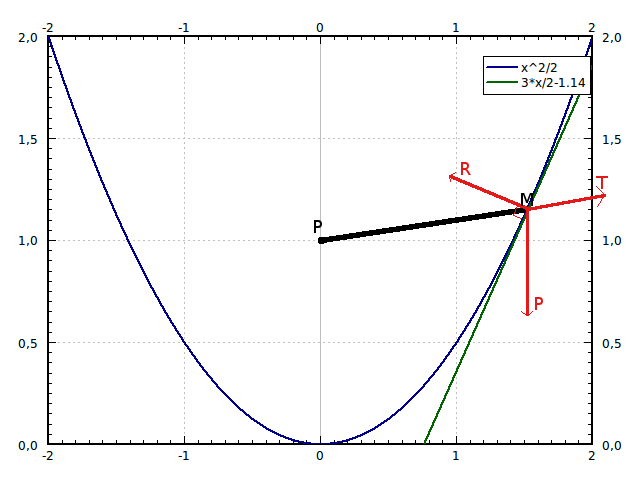
\includegraphics[scale=0.7]{GraphMath2.png}
	%\caption{Histoire de Sanofi}
\end{figure}
La masselotte M se déplace uniquement selon la composante tangentielle. Pour déterminer l'équation différentielle on va donc particulièrement s'intéresser à l'équation sur la composante tangentielle.\\
Pour cela, étudie la somme des forces s'exerçant sur la composante tangentielle $\vec{u_t}$ et normale $\vec{u_n}$. Selon la seconde loi de Newton (PFD) :
\[
   \left \{
   \begin{array}{r c l}
      P_t+T_t=ma_t  \\
      P_n+R_n+T_n=0 
   \end{array}
   \right .
\]
On s'intéresse à l'équation: \[\fbox{$P_t+T_t=ma_t$}\] \\ 
Pour déterminer l'équation différentielle, on doit alors projeter $\vec{T}$ et  $\vec{mg}$ sur $\vec{u_t}$. \\

\subsection{Projection du Poids sur la composante tangentielle}
On projette $\vec{mg}=-mg.\vec{u_y}$ sur $\vec{u_t}$\\
\begin{figure}[H]
	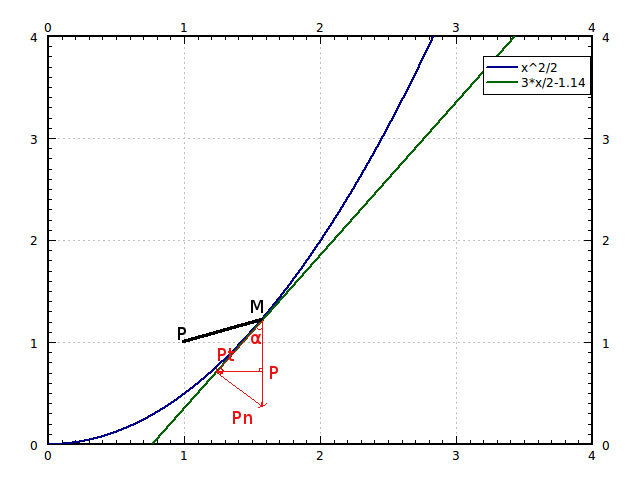
\includegraphics[scale=0.7]{GraphMathZoomProjectionPoids.png}
	%\caption{Histoire de Sanofi}
\end{figure}

On projette tel que $P_t=P.\cos(\alpha)$\\
On cherche à déterminer $\alpha$.
On calcule la pente a de la tige parabolique. $a=\frac{\partial y}{\partial x}=\frac{\partial x^2/2}{\partial x}=x$ \\
En $M(x_0,y_0)$ la pente a de la tige parabolique vaut donc $x_0$.
Cette pente permet de calculer l'angle $\alpha$. En effet, on remarque graphiquement que $\tan(\alpha)=\frac{1}{a}$.\\
On en déduit: $\alpha=\tan^{-1}(\frac{1}{x_0})$\\
$P_t=P.\cos(\tan^{-1}(\frac{1}{x_0})) $\\
Or $\cos(\tan^{-1}(x))=\frac{1}{\sqrt{1+x^2}}$\\
On en déduit donc: $P_t=P.\frac{1}{\sqrt{1+1/x^2_0}}$\\
D'où: 
\[\fbox{$P_t=P.\frac{x_0}{\sqrt{1+x^2_0}}$}\]

\subsection{Projection de la tension du ressort su la composante tangentielle}
On projette désormais $\vec{T}$ sur $\vec{u_t}$.\\

\begin{figure}[H]
	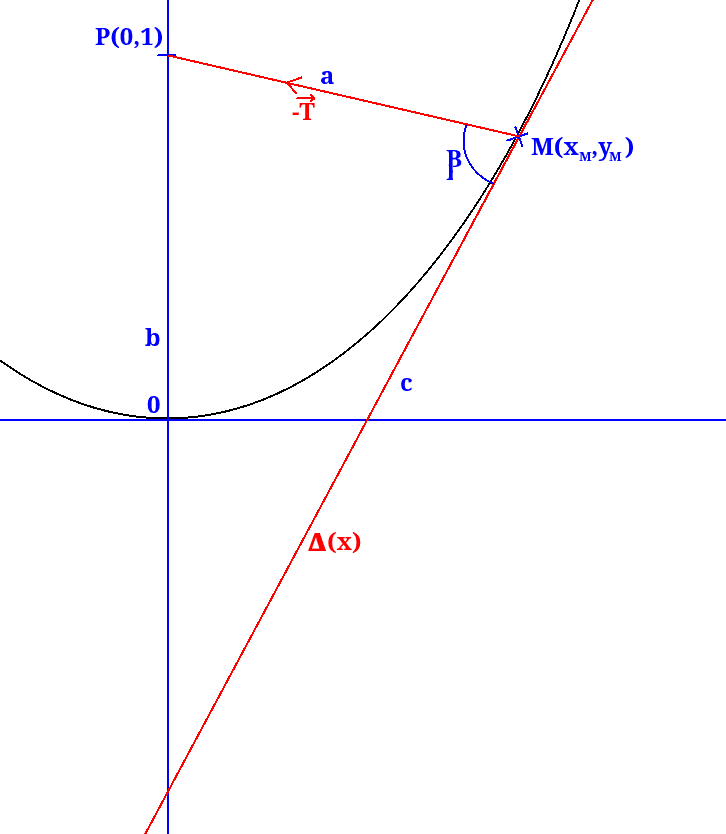
\includegraphics[scale=0.5]{al-kashi.png}
	%\caption{Histoire de Sanofi}
\end{figure}
On note x,y les coordonnées du point M. D'après le théorème de Pythagore :\\
$a=\sqrt{(x_M-x_P)^2+(y_M-y_P)^2}=\sqrt{x^2+(\frac{x^2}{2}-1)}=\sqrt{x^2+\frac{x^4}{4}-x^2+1}=\sqrt{\frac{x^4}{4}+1}$\\
$b=\sqrt{(x_M-x_P)^2+(y_M-\Delta(0))^2}=\sqrt{x^2+(\frac{x^2}{2}+\frac{x^2}{2})^2}=\sqrt{x^2+x^4}=|x|\sqrt{1+x^2}$\\
$c=\sqrt{(y_p-\Delta(0))^2}=\sqrt{(1+\frac{x^2}{2})^2}=1+\frac{x^2}{2}$\\
D'après le théorème d'Al-Kashi : \\
$c^2 = a^2 + b^2 - 2ab\times\cos(\beta)$\\
$\cos(\beta)=\frac{a^2+b^2-c^2}{2ab}=\frac{x^4/4+1+x^2+x^4-1-x^2-x^4/4}{2x\sqrt{x^4/4+1}\sqrt{1+x^2}}=\frac{x^3}{2\sqrt{\frac{x^4}{4}+1}\sqrt{1+x^2}}$\\
On trouve donc :
\[\fbox{ $T_t=T\times\frac{x^3}{2\sqrt{\frac{x^4}{4}+1}\sqrt{1+x^2}}$ }\]\\

\subsection{Determination de $ \|T\| $}
On détermine la valeur de la tension du ressort.\\
$T=k(l-l_0)=k(\sqrt{(x_M-x_P)^2+(y_M-y_P)^2}-l_0)=k(\sqrt{x^2+(x^2/2-1)^2}-l_0)$\\
$T=k(\sqrt{x^2+x^4/4-x^4+1}-l_0)$\\
\[\fbox{ $T=k(\sqrt{1+\frac{x^4}{4}}-l_0)$ }\]

\subsection{Détermination de $a_t$}
On a vu dans la première équation que $a_n=0$. On en déduit: $||\vec{a}||=a_t$\\
Avec une accélération normale nulle, on peut écrire la formule de l'accélération dans le repère de Frenet ainsi : $a_t=||\vec{a}||$\\ %=$\sqrt{a_x^2+a_y^2}$
Or $||\vec{a}||=\frac{\partial v}{\partial t}=\frac{\partial \pm\sqrt{\dot{x}^2+\dot{y}^2}}{\partial t}$\\
$ \dot{y}=\frac{\partial y}{\partial t}=\frac{\partial y}{\partial x}\times\frac{\partial x}{\partial t}=x\dot{x} $\\
$ v=\sqrt{\dot{x}^2+\dot{x}^2x^2}=\dot{x}\sqrt{1+x^2} $\\
$ \frac{\partial v}{\partial t}=\ddot{x}\sqrt{1+x^2}+\frac{\dot{x}^2x}{\sqrt{1+x^2}} $\\
On trouve: \[\fbox{$a_t=\ddot{x}.\sqrt{1+x^2}+ \frac{\dot{x}^2.x}{\sqrt{1+x^2}}$}\]
%On obtient alors: $a_t=\sqrt{\ddot{x}^2+\ddot{y}^2}$

\subsection{Détermination de l'équation différentielle}
A l'aide de ce qu'on a calculé précédemment on développe l'équation $mg_t+T_t=ma_t$ pour déterminer l'équation différentielle.
%On obtient alors: 
%\subsubsection{Equa diff de Guillaume}
%En développant et en prenant k=m, g=1 et $a=l_0$ (données de l'énoncé), on obtient :\\
%$m.1.\frac{x}{\sqrt{1+x^2}} + m(\sqrt{x^4/4+1}-a).[\frac{1}{\sqrt{1+x^2}}.\frac{x}{\sqrt{1+x^4/4}} + \sqrt{1-\frac{1}{1+x^2}}.\sqrt{1-\frac{x^2}{1+x^4/4}}] - m.\ddot{x}.\sqrt{1+x^2} - m.\frac{\dot{x}^2.x}{\sqrt{1+x^2}} = 0$ \\
% 
%$\frac{x}{\sqrt{1+x^2}} + (\sqrt{x^4/4+1}-a).[\frac{1}{\sqrt{1+x^2}}.\frac{x}{\sqrt{1+x^4/4}} + \sqrt{1-\frac{1}{1+x^2}}.\sqrt{1-\frac{x^2}{1+x^4/4}}] - \ddot{x}.\sqrt{1+x^2} - \frac{\dot{x}^2.x}{\sqrt{1+x^2}} = 0$
%  
%$\frac{x}{\sqrt{1+x^2}} + (\sqrt{x^4/4+1}-a).[\frac{1}{\sqrt{1+x^2}}.\frac{x}{\sqrt{1+x^4/4}} + \frac{x}{\sqrt{1+x^2}}.\sqrt{\frac{x^4/4-x^2+1}{1+x^4/4}}] - \ddot{x}.\sqrt{1+x^2} - \frac{\dot{x}^2.x}{\sqrt{1+x^2}} = 0$
%  
%$\frac{x}{\sqrt{1+x^2}} + [\frac{x}{\sqrt{1+x^2}} + \frac{x.\sqrt{x^4/4-x^2+1}}{\sqrt{1+x^2}}] -a.[\frac{1}{\sqrt{1+x^2}}.\frac{x}{\sqrt{1+x^4/4}} + \frac{x}{\sqrt{1+x^2}}.\sqrt{\frac{x^4/4-x^2+1}{1+x^4/4}}] - \ddot{x}.\sqrt{1+x^2} - \frac{\dot{x}^2.x}{\sqrt{1+x^2}} = 0$
% 
%$\frac{x}{1+x^2} + [\frac{x}{1+x^2} + \frac{x.\sqrt{x^4/4-x^2+1}}{1+x^2}] -a.[\frac{x}{(1+x^2).\sqrt{1+x^4/4}} +\frac{x.\sqrt{x^4/4-x^2+1}}{(1+x^2).\sqrt{1+x^4/4}}] - \ddot{x} - \frac{\dot{x}^2.x}{1+x^2} = 0$
%
%$\frac{2x+x.\sqrt{x^4/4-x^2+1}-\dot{x}^2.x}{1+x^2} -a.\frac{x+x.\sqrt{x^4/4-x^2+1}}{(1+x^2).\sqrt{1+x^4/4}} - \ddot{x}= 0$
%
%$-\frac{2x+x.\sqrt{x^4/4-x^2+1}-\dot{x}^2.x}{1+x^2} +a.\frac{x+x.\sqrt{x^4/4-x^2+1}}{(1+x^2).\sqrt{1+x^4/4}} + \ddot{x}= 0$
%
%$-\frac{2x+x.\sqrt{(x^2/2-1)^2}-\dot{x}^2.x}{1+x^2} +a.\frac{x+x.\sqrt{(x^2/2-1)^2}}{(1+x^2).\sqrt{1+x^4/4}} + \ddot{x}= 0$
%
%\[ \fbox{$\frac{-x^3/2-x+\dot{x}^2x}{1+x^2} + \frac{a.x^3}{2(1+x^2).\sqrt{1+x^4/4}} + \ddot{x}= 0$} \]
%  
%  
%% \[mg.\cos(\tan^{-1}(x_0)) + k(l-l_0).\cos(\tan^{-1}(x_0) - \tan^{-1}(\frac{y_0-1}{x_0}))=\sqrt{\ddot{x}^2+\ddot{y}^2}\]
% %En développant on a:\[mg.\cos(\tan^{-1}(x)) + k(\sqrt{(x^2/2-1)^2+x^2}-l_0).\cos(\tan^{-1}(x) - \tan^{-1}(\frac{x^2/2-1}{x})) - \sqrt{\ddot{x}^2+1}=0\]
%
%\subsubsection{Equa diff de Charles}
On calcule maintenant l'équatio ndifférentielle du système en s'aidant des résultats précédents.\\
On part de l'équation $ P_t+T_t=ma_t $\\
avec $T_t=k(l-l_0)$ et $P_t=-mg$\\
En développant les expression on obtient :\\
$-k(\sqrt{x^4/4+1}-l_0)\times \frac{x^3}{2\sqrt{x^4/4+1}\sqrt{1+x^2}}-mg\frac{x}{\sqrt{1+x^2}}=m(\ddot{x}\sqrt{1+x^2}+\frac{\ddot{x}^2x}{\sqrt{1+x^2}})$\\
$ -\frac{k}{m}(\frac{x^3}{2\sqrt{1+x^2}}-\frac{x^3\times l_0}{2\sqrt{x^4/4+1}\sqrt{1+x^2}})-\frac{xg}{\sqrt{1+x^2}}-\ddot{x}\sqrt{1+x^2}-\frac{\dot{x}^2x}{\sqrt{1+x^2}}=0 $\\
En prenant k=m, g=1 et $a=l_0$ (données de l'énoncé), on obtient :\\
$ -\frac{x^3}{2\sqrt{1+x^2}}+\frac{x^3\times a}{2\sqrt{x^4/4+1}\sqrt{1+x^2}}-\frac{x}{\sqrt{1+x^2}}-\ddot{x}\sqrt{1+x^2}-\frac{\dot{x}^2x}{\sqrt{1+x^2}}=0 $\\
$\frac{x^3}{2\sqrt{1+x^2}}-\frac{a x^3}{2\sqrt{1+x^4/4}\sqrt{1+x^2}}+\frac{x}{\sqrt{1+x^2}}+\ddot{x}\sqrt{1+x^2}+\frac{\dot{x}^2x}{\sqrt{1+x^2}}=0$\\
L'équation différentielle revient donc à :\\
\[ \fbox{$ \ddot{x} + \frac{\dot{x}^2 x}{1+x^2} + \frac{x^3}{2(1+x^2)} - \frac{ax^3}{2\sqrt{1+x^4/4}(1+x^2)} + \frac{x}{1+x^2} = 0 $}\]

\section{Dans toute la suite on supposera que g=1, k=m et on notera $a=l_0$ et on s'intéressera particulièrement par l'équation vérifié par x(t).}
\subsection{Montrer que l'équation est de la forme: $\ddot{x} + f(x,\dot{x},a) = 0.$}
On retrouve la forme $\ddot{x} + f(x,\dot{x},a) = 0$, avec $f(x,\dot{x},a)=\frac{\dot{x}^2x+x^3/2+x}{1+x^2}-\frac{x^3\times a}{2\sqrt{x^4/4+1}(1+x^2)}$ 
\subsection{Détermination des points d'équilibre}

Les points d'équilibre sont les points où la vitesse du système et donc de la masselotte est nulle. Ainsi, les tèrmes lié à la vitesse et à l'accélération du système sont nuls.\\
Les points d'équilibres correspondent aux solutions de l'équation :\\
$ \ddot{x}+\frac{\dot{x}^2x-x^3/2-x}{1+x^2}+\frac{x^3\times a}{2\sqrt{x^4/4+1}(1+x^2)}=0 $
où 
$\ddot{x}=0$ et $\dot{x}=0$ aux points d'équilibre.\\
Ce qui revient à l'équation :\\
$\frac{-x^3/2-x}{1+x^2} + \frac{x^3\times a}{2\sqrt{x^4/4+1}(1+x^2)}=0$ \\
Une première solution correspond à $x_0=0$ et $y_0=0$ \\
En multipliant de part et d'autre de l'équation par $\frac{2(1+x^2)}{x}$ :\\
$x^2-\frac{x^2\times l_0}{\sqrt{1+x^4/4}}+2=0$\\
$\sqrt{1+x^\frac{4}{4}}(x^2+2)=x^2\times l_0$\\
$\sqrt{1+y^2}(2y+2)=2yl_0$\\
$(1+y^2)(4y^2+8y+4)=4y^2\times l_0^2$\\
$(1+y^2)(y^2+2y+1)=y^2\times l_0^2$\\
$(\frac{1}{y}+y)(y+2+\frac{1}{y})=l_0^2$\\
On pose $X=y+\frac{1}{y}$ ($y\neq 0$):\\
$X(X+2)=l_0^2$\\
$X^2+2X-l_0^2=0$\\
Dont on calcule le déterminant :
$\Delta_X=4(1+l_0^2)$\\
D'où les solutions intermédiaires :
$X_1=-1-\sqrt{1+l_0^2}$\\
$X_2=-1+\sqrt{1+l_0^2}$\\
$y+\frac{1}{y}=X$\\
$y^2+1=Xy$\\
$y^2-Xy+1=0$\\
Dont le déterminant est :
$\Delta_y=X^2-4$\\
D'où les solutions :\\
$y=\frac{1}{2}(X-\sqrt{X^2-4})$\\
$y=\frac{1}{2}(X+\sqrt{X^2-4})$\\
Cependant, il faut savoir que $\Delta_y$ doit être positif afin que les racines soient rélles.\\

\renewcommand{\labelitemi}{$\circ$}

Pour la solution $X=(-1+\sqrt{1+l_0^2})^2$, nous avons deux cas de condition d'existance :\\
\begin{itemize}
\item $(-1+\sqrt{1+l_0^2})^2 > 2 \Rightarrow \sqrt{1+l_0^2}>3\Rightarrow l_0 > \sqrt{8}$
\item $(-1+\sqrt{1+l_0^2})^2 < -2 \Rightarrow \sqrt{1+l_0^2}<-1$ qu iest une condition irréalisable
\end{itemize}
Finalement, on déduit que la condition d'existence des points d'équilibres est $l_0>\sqrt{8}$.
On peut alors trouver l'expression des ordonnées des points d'équilibre $y_1,y_2,y_3,y_4$ en fonction de $l_0$ :\\
\begin{itemize}
\item $y_0=0$\\
(Déterminé précédemment)\\
\item $y_1=\frac{1}{2}(X_1-\sqrt{X_1-4})=\frac{1}{2}(-1-\sqrt{1+l_0^2})-\frac{1}{2}(\sqrt{(-1-\sqrt{1+l_0^2})^2-4})$\\
%$=\frac{1}{2}(-1-\sqrt{1+l_0^2})-\frac{1}{2}\sqrt{1+2\sqrt{1+l_0^2}+(1+l_0^2)-4}$\\
%$=\frac{1}{2}(-1-\sqrt{1+l_0^2})-\frac{1}{2}\sqrt{-2+2\sqrt{1+l_0^2}+l_0^2}$\\
Cette solution est strictement négative alors que y(t) est positive, selon la rampe $y=\frac{x^2}{2}$. On doit alors l'éliminer.\\
\item $y_2=\frac{X_1+\sqrt{X_1-4}}{2}=\frac{1}{2}(-1-\sqrt{1+l_0^2})+\frac{1}{2}\sqrt{-2+2\sqrt{1+l_0^2}+l_0^2}$\\
Cette solution est aussi à éliminer. En effet, nous avons : \\
$y_2 >0 \Rightarrow (-1-\sqrt{1+l_0^2}+\sqrt{(-1-\sqrt{1+l_0^2})^2+l_0^2} > 0$\\$\Rightarrow \sqrt{(-1-\sqrt{1+l_0^2})^2+l_0^2}>1+\sqrt{1+l_0^2}$\\$ \Rightarrow 0>\sqrt{1+l_0^2}$ ce qui est impossible.
\item $y_3=\frac{X_2-\sqrt{X_2-4}}{2}=\frac{1}{2}(-1+\sqrt{1+l_0^2})-\frac{1}{2}\sqrt{(-1+\sqrt{1+l_0^2})^2-4}$\\
%$=\frac{1}{2}(-1+\sqrt{1+l_0^2})-\frac{1}{2}\sqrt{1-2\sqrt{1+l_0^2}+(1+l_0^2)-4}$\\
$=\frac{1}{2}(-1+\sqrt{1+l_0^2})-\frac{1}{2}\sqrt{-2-2\sqrt{1+l_0^2}+l_0^2}$\\
\item $y_4=\frac{1}{2}(-1+\sqrt{1+l_0^2})+\frac{1}{2}\sqrt{(-1+\sqrt{1+l_0^2})^2-4}$\\
$=\frac{1}{2}(-1+\sqrt{1+l_0^2})+\frac{1}{2}\sqrt{-2-2\sqrt{1+l_0^2}+l_0^2}$\\
\end{itemize}
Seules deux solutions sont alors retenues, l'unique condition d'existance étant $l_0>\sqrt{8}$.\\
En considérant $y=\frac{x^2}{2} \Longrightarrow x=\pm \sqrt{2y}$ on a au total 5 points d'équilibre :\\
$x_0=0$\\
$x_1=\sqrt{-1+\sqrt{1+l_0^2}-\sqrt{-2-2\sqrt{1+l_0^2}+l_0^2}})$\\
$x_2=-\sqrt{-1+\sqrt{1+l_0^2}-\sqrt{-2-2\sqrt{1+l_0^2}+l_0^2}})$\\
$x_3=\sqrt{-1+\sqrt{1+l_0^2}+\sqrt{-2-2\sqrt{1+l_0^2}+l_0^2}}$\\
$x_4=-\sqrt{-1+\sqrt{1+l_0^2}+\sqrt{-2-2\sqrt{1+l_0^2}+l_0^2}}$\\
Il reste à déterminer la nature de ces points d'équilibre du système.

\subsection{Détermination de la nature des points d'équilibre}
Nous sommes dans le cas d'un système non linéaire.
On pose $x_1=x, x_2=\dot{x}$\\
On a alors :
\[\dot{x_1}=x_2=f_1(x_1*,x_2*)\]
\[ \dot{x_2}=-\frac{x^2_2.x_1}{1+x^2_1} - \frac{x^3_1}{2(1+x^2_1)} - \frac{x_1}{1+x^2_1} + \frac{ax^3_1}{2(1+x^2_1)(x^4_1/4 + 1)}=f_2(x_1,x_2) \]



Aux points d'équilibre, la vitesse est nulle d'où $x_2=0$ et $\dot{x_2}=0$\\
D'où :\\
\[ f_1(x_1*,0) = 0 \]
\[ f_2(x_1*,0) = \frac{x_1^3\times l_0}{2\sqrt{1+\frac{x_1^4}{4}}(1+x_1^2)}-\frac{x_1^3}{2(1+x_1^2)} - \frac{x}{1+x^2} \]

On va calculer la nature des points d'équilibre en passant par la matrice Jacobienne :\\
\[
J=
\begin{pmatrix}
\frac{\delta f_1}{dx_1} & \frac{\delta f_1}{dx_2} \\
\frac{\delta f_2}{dx_1} & \frac{\delta f_2}{dx_2}
\end{pmatrix}
=
\begin{pmatrix}
0&1\\
\frac{\delta f_2}{dx_1}&0
\end{pmatrix}
\]

La nature des points d'équilibre du système est définie par la trace, le déterminant, et le discriminant du polynôme caractéristique de la matrice Jacobienne ci-dessus.\\
$ Tr(J) = 0 $\\
$ det(J) = -\frac{\delta f_2}{\delta x_1} $\\
$ \Delta(J) = Tr^2(J) - 4det(J) = 4*\frac{\delta f_2}{\delta x_1} $\\

On a alors besoin de déterminer le signe de $frac{\delta f_2}{\delta x_1}$ aux points d'équilibre.\\

En factorisant $f_2$, on a : \\
$f_2=0=-\frac{x}{2(1+x^2)}*(x^2-\frac{x^2\times l_0}{\sqrt{1+\frac{x^4}{4}}}+2)$\\
car $\ddot{x} = 0$ aux points d'équilibre.\\

Ici, nous avons deux éventualités pour satisfaire cette équation :\\
\begin{itemize}
\item cas 1 : $\frac{x}{1+x^2}=0$\\
\item cas 2 : $x^2-\frac{x^2\times l_0}{\sqrt{1+\frac{x^4}{4}}}+2=0$\\
\end{itemize}

\subsubsection*{Premier Cas}
$\frac{x}{1+x^2}=0 \longrightarrow x=0$\\
On a alors :\\
$\frac{\delta f_2}{\delta x_1}=\frac{-1}{2}\frac{\delta \frac{x}{1+x^2}}{\delta x}(x^2 - \frac{x^2\times l_0}{\sqrt{1+\frac{x^4}{4}}}+2)=-2\frac{1+x^2-4x^2}{2(1+x^2)^2}$
Ce qui équivaut, avec l'hypothèse précédente $x=0$, à :\\
\[frac{\delta f_2}{\delta x_1}=-1\]

La matrice jacobienne du système pour le point d'équilibre $x=0$ devient donc :\\
\[
J=
\begin{pmatrix}
0&1\\
-1&0
\end{pmatrix}
\]
On peut alors en calculer les caractéristique :\\
$tr(J_f) = 0 $\\
$det(J_f) =  1 $\\
$\Delta(J_f) = -4$\\
Ce sont les caractéristiques d'un point d'équilibre centré.\\

\subsubsection*{Second Cas}
Dans ce cas, $x^2-\frac{x^2\times l_0}{\sqrt{1+\frac{x^4}{4}}}+2=0$\\
On a alors :\\
$\frac{\delta f_2}{\delta x}=-\frac{x}{2(1+x^2)}(2x-\frac{2x\times l_0\sqrt{1+\frac{x^4}{4}}-x^2\times l_0\frac{x^3}{2\sqrt{1+\frac{x^4}{4}}}}{1+\frac{x^4}{4}})=
-\frac{x}{2(1+x^2)}(2-\frac{2\times l_0}{\sqrt{1+\frac{x^4}{4}}}+l_0\frac{x^4}{2\sqrt{1+\frac{x^4}{4}^{3/2}}})$\\$= \frac{-x^2}{2(1+x^2)}\frac{2(1+\frac{x^4}{4})-\frac{2}{x^2}(2+x^2)(1+\frac{x^4}{4})+\frac{x^2}{2}(2+x^2)}{1+\frac{x^4}{4}}=\frac{-x^2+2}{(1+x^2)(1+\frac{x^4}{4})}=\frac{(x-\sqrt{2})(x+\sqrt{2})}{(1+x^2)(1+\frac{x^4}{4})}$\\
Etudier le signe de $\frac{\delta f_2}{\delta x}$ revient donc à étudier le signe de $-x^2+2$.\\
On en calcule alors le discriminant pour connaitre les solutions pour dresser, par la suite, un tableau de variation.
$\Delta = 8$\\
D'où les solutions :\\
$x_1 = -\frac{\sqrt{8}}{-2} = -\sqrt{2}$\\
$x_2 = \frac{\sqrt{8}}{-2} = \sqrt{2}$\\
D'où le tableau de variations suivant :\\
\begin{tikzpicture}
%\tkzTab{$x$/1,$\frac{\delta f_2}{\delta x_1}$/1,$f_2$/1.8}{$-\infty$,$+\infty$}{+,-,+}{-/$-\infty$, +/$+\infty$}
%\tkzTabVal[draw]{1}{2}{0.3}{$-\sqrt{2}$}{$0$}
%\tkzTabVal[draw]{1}{2}{0.7}{$\sqrt{2}$}{$0$}\\
\tkzTab{$x$/1,$\frac{\delta f_2}{\delta x_1}$/1}{$-\infty$,$+\infty$}{+,-,+}{,}
\tkzTabVal[]{1}{2}{0.3}{$-\sqrt{2}$}{}
\tkzTabVal[]{1}{2}{0.7}{$\sqrt{2}$}{}\\
\end{tikzpicture}\\
\\
Avec $\frac{\delta f_2}{\delta x_1}=0$ pour $x=\pm \sqrt{2}$.
Les points d'équilibre sont les suivants :\\
%%%%%%%%%%%%%%%%%%%%%%%%%%%%
$x=0$\\
$x_1=\sqrt{-1+\sqrt{1+l_0^2}-\sqrt{-2-2\sqrt{1+l_0^2}+l_0^2}})$\\
$x_2=-\sqrt{-1+\sqrt{1+l_0^2}-\sqrt{-2-2\sqrt{1+l_0^2}+l_0^2}})$\\
$x_3=\sqrt{-1+\sqrt{1+l_0^2}+\sqrt{-2-2\sqrt{1+l_0^2}+l_0^2}}$\\
$x_4=-\sqrt{-1+\sqrt{1+l_0^2}+\sqrt{-2-2\sqrt{1+l_0^2}+l_0^2}}$\\
%%%%%%%%%%%%%%%%%%%%%%%%%%%%

On peut alors étudier leur nature.\\
\subsubsection*{Nature des points d'équilibre}
En partant de la condition d'existence des points d'équilibre:\\
$l_0>2\sqrt{2}$\\
$1+l_0^2>9$\\
$-1+\sqrt{1+l_0^2}>2$\\
avec :\\
$\sqrt{(-1+\sqrt{1+l_0^2})^2-4}>0$\\
Ce qui nous permet enfin de calculer la nature des points d'équilibre :
\begin{itemize}
\item $x_0=0$\\
D'après le tableau de variation, $\frac{\delta f_2}{\delta x}$<0.\\
$tr(J_f) = 0 $\\
$det(J_f) > 0 $\\
$\Delta(J_f) < 0$\\
Il s'agit d'un point centre.
\item $x_1=\sqrt{-1+\sqrt{1+l_0^2}-\sqrt{-2-2\sqrt{1+l_0^2}+l_0^2}})$\\
Correspondant à : $y_3=\frac{1}{2}(-1+\sqrt{1+l_0^2})-\frac{1}{2}\sqrt{(-1+\sqrt{1+l_0^2})^2-4}$\\
On pose :\\
$A=-1+\sqrt{1+l_0^2}$\\
$B=\sqrt{(-1+\sqrt{1+l_0^2})^2-4} = \sqrt{A^2-4}$\\
$y=\frac{1}{2}(A-B)$\\
D'après le théorème des trois maisons, on a :\\
$B > \sqrt{A^2} - \sqrt{4}$\\
$B > A - 2$\\
$A-B < 2$\\
$\frac{1}{2}(A-B)<1$\\
$y_3 < 1$\\
$\frac{x_1^2}{2}<1$\\
$x_1^2<2$\\
D'où :
$x_1<\sqrt{2}$ et $x_1>-\sqrt{2}$\\
D'après le tableau de variations, $\frac{\delta f_2}{\delta x_1}<0$. Ainsi :\\
$tr(J_f) = 0 $\\
$det(J_f) > 0 $\\
$\Delta(J_f) < 0$\\
Il s'agit d'un point centre.
\item $x_2=-\sqrt{-1+\sqrt{1+l_0^2}-\sqrt{-2-2\sqrt{1+l_0^2}+l_0^2}})$\\
Il s'agit de l'opposé de $x_1$, on est donc aussi dans le cas de $\frac{\delta f_2}{\delta x_1}<0$.\\
$x_2$ est donc, comme $x_1$, un point centre.
\item $x_3=\sqrt{-1+\sqrt{1+l_0^2}+\sqrt{-2-2\sqrt{1+l_0^2}+l_0^2}}>\sqrt{2}$\\
Car racine carrée d'une somme de expressions supérieures à zéro, dont l'une supérieur à 2.
D'après le tableau de variation, $\frac{\delta f_2}{\delta x}>0$. Ainsi :\\
$tr(J_f) = 0 $\\
$det(J_f) < 0 $\\
$\Delta(J_f) > 0$\\
Il s'agit d'un point selle.
\item $x_4=-\sqrt{-1+\sqrt{1+l_0^2}+\sqrt{-2-2\sqrt{1+l_0^2}+l_0^2}}<-\sqrt{2}$\\
Puisqu'il s'agit de l'opposé de $x_3$.
D'après le tableau de variation, $\frac{\delta f_2}{\delta x}>0$.\\
$x_4$ est donc, comme $x_3$, un point selle.\\
\end{itemize}
On représente les $x_n$ sur le portrait de phase.
%LA CE SERAIT SYMPA DE FAIRE UN SCHEMA AVEC EN GROS LES Xn PLACÉS A PEU PRES.


%D'après l'équation:\\
%$\ddot{x}=0$\\
%On a :\\
%$\sqrt{1+\frac{x^4}{4}}=\frac{x^2\times l_0}{2+x^2}$\\
%On peut alors simplifier l'équation de la dérivée partielle de $f_2$, pour obtenir :\\
%$\frac{\delta f_2}{\delta x}=-\frac{x}{2(1+x^2)}(2-\frac{2(2+x^2}{x^2}+\frac{x^2}{2}\frac{2+x^2}{1+\frac{x^4}{4}})$
%
%Pour étudier le signe de $\frac{\delta f_2}{\delta x}$, on la compare à 0 :
%$2x^2-2(2+x^2)+\frac{x^4}{4}\frac{2+x^2}{1+\frac{x^4}{4}}=0$\\
%$2x^2-\frac{x^6}{2}-(4+2x^2)(1+\frac{x^4}{4})+x^4+\frac{x^6}{2}=0$\\
%$2x^2+x^6-4-x^4-2x^2-\frac{x^6}{2}+x^4=0$\\
%$\frac{x^6}{2}-4=0$\\
%$x^6=8$\\
%On peut alors déterminer le signe de $\frac{\delta f_2}{\delta x}$ qui est directement lié à celui de $x^6-8$, afin de trouver le signe de :\\
%$tr(J_f) = 0 $\\
%$det(J_f) =  -C\times(x^6-8) $\\
%$\Delta(J_f) = 4C\times(x^6-8)$\\
%Avec C une fonction strictement positive.
%
%Les relations qui lient le signe de $\frac{\delta f_2}{\delta x_1}$ à celui de $x^6-8$ sont les suivantes :\\
%$\frac{\delta f_2}{\delta x_1}<0$ si $x^6<8$\\
%$\frac{\delta f_2}{\delta x_1}=0$ si $x^6=8$\\
%$\frac{\delta f_2}{\delta x_1}>0$ si $x^6>8$\\

%Il faut alors déterminer $\frac{\delta f_2}{dx_1}$ : \\
%\[ \frac{\delta f_2}{dx_1} = \frac{3l_0x_1^2+l_0x^4 - (1+x^2)\frac{l_0x^6}{2(1+\frac{x^4}{4})}}{2\sqrt{1+\frac{x^4}{4}}(1+x^2)^2}-\frac{3x^2+x^4}{2(1+x^2)^2} \]
%Détail du calcul de  $\frac{\delta f_2}{dx_1}$ :\\
%(VIDE !!! voir lune à plume, je vois de quoi je parle. Pour info, c'est du calcul brut, pas "d'astuce")\\
%
%On peut alors calculer les propriétés de la matrice (respectivement Déterminant, Trace, Discriminant du polynôme caractéristique) :\\
%\[ det(J_f) =  \frac{\delta f_2}{dx_1} \]
%\[ tr(J_f) = 0 \]
%\[ \Delta(J_f) = tr(J_f)^2 - 4\times det(J_f) = 4\frac{\delta f_2}{dx_1}\]
%Pour connaitre la nature du point d'équilibre, il nous reste plus qu'à étudier le signe de $\frac{\delta f_2}{dx_1}$ :\\
%\[ \frac{\delta f_2}{dx_1} = \frac{3l_0x_1^2+l_0x^4 - (1+x^2)\frac{l_0x^6}{2(1+\frac{x^4}{4})}}{2\sqrt{1+\frac{x^4}{4}}(1+x^2)^2}-\frac{3x^2+x^4}{2(1+x^2)^2} \]
%D'après la question précédente, on a en tout point d'équilibre $\sqrt{1+\frac{x^4}{4}}=\frac{x^2l_0}{x^2+2}$, d'où : \\
%\[ \frac{\delta f_2}{dx_1} = \frac{3l_0x_1^2+l_0x^4 - \frac{1}{2}(x^2+2)^2(1+x^2)\frac{l_0x^6}{\frac{(x^2l_0)^2}{(x^2+2)}}}{2(1+x^2)^2}-\frac{3x^2+x^4}{2(1+x^2)^2} \]
%\[ =\frac{-\frac{1}{2l_0}x^2(x^2+2)^2(1+x^2)(x^2+2)+(3l_0x^2+l_0x^2+l_0x^4)(x^2+2)-3x^2-x^4}{2(1+x^2)^2} \]
%
%(Jusqu'à là, je suis sur que c'était la bonne méthode. Le remplacement de $\sqrt{1+\frac{x^4}{4}}=\frac{x^2l_0}{x^2+2}$ est lui-aussi bon) \\
%
%Le dénominateur étant positif pour tout x, on cherche le signe du numérateur, c-à-d de :\\
%\[ -\frac{1}{2l_0}x^2(x^2+2)^2(1+x^2)(x^2+2)+(3l_0x^2+l_0x^2+l_0x^4)(x^2+2)-3x^2-x^4 \]
%
%%Thibault:
%Étude de signe du polynôme:\\
%on pose, \[ -\frac{1}{2l_0}x^2(x^2+2)^2(1+x^2)(x^2+2)+(3l_0x^2+l_0x^2+l_0x^4)(x^2+2)-3x^2-x^4  = 0\]
%
%Le polynôme est factorisable par $x^2$ et on obtient un polynôme d'ordre 8\\
%$-1x^8/l_0-7x^6/l_0-18x^4/l_0+x^2(n 6l_0-1-20/l_0)+(8l_0-1-8l_0) = 0$\\
%On pose :\\ $V = -1/l_0$\\   $Y = (6l_0-1-20/l_0)$\\   $Z = (8l_0-1-8/l_0)$\\
%on a: $Vx^8+7Vx^6+18Vx^4+Yx^2+Z = 0$\\
%le polynôme est d'ordre 8 c'est donc un ordre pair donc il admet au maximum deux racines.\\
%Or le coefficient de l'ordre 8 est impair et z est négatif donc le polynôme admet deux racines de signes contraires.\\
%on peut donc factoriser le polynôme par un polynôme d'ordre 6 et par un polynôme d'ordre 2\\










\section{On suppose que $a=\sqrt{15}$.}
\subsection{Déterminer la valeur exacte des points d'équilibres du système.}
On détermine les valeurs numériques des points d'équilibres pour $a=\sqrt{15}$. On a:\\
$x_0=0$\\
$x_1=\sqrt{3 - \sqrt{5}}=0.874$\\
$x_2=\sqrt{3 - \sqrt{5}}=-0.874$\\
$x_3=-\sqrt{3 + \sqrt{5}}=2.288$\\
$x_4=-\sqrt{3 + \sqrt{5}}=-2.288$\\

\subsection{Déterminer l'intégrale première du système.}
	On rappelle que $v=\dot{x}\sqrt{1 + x^2}$ et $\frac{\delta{v}}{\delta{t}}=\ddot{x}\sqrt{1 + x^2} + \frac{\dot{x}^2.x}{\sqrt{1+x^2}}$ \\
On va intégrer cette équation différentielle.
\[  \ddot{x}+\frac{\dot{x}^2x}{1+x^2} + \frac{1}{2}\frac{x^3}{1+x^2} + \frac{x}{1+x^2} - \frac{a.x^3}{2(1+x^2)\sqrt{x^4/4+1}}=0 \]	
On multiplie cette équation par $\sqrt{1+x^2}$:

\[  \ddot{x}\sqrt{1+x^2}+\frac{\dot{x}^2x}{\sqrt{1+x^2}} + \frac{1}{2}\frac{x^3}{\sqrt{1+x^2}} + \frac{x}{\sqrt{1+x^2}} - \frac{a.x^3}{2\sqrt{1+x^2}\sqrt{x^4/4+1}}=0 \]	

On remarque ainsi que l'équation s'écrit de la forme:\\
\[ \frac{\delta{v}}{\delta{t}} + \sqrt{1+x^2}f(x) = 0 \] avec $f(x)=  \frac{1}{2}\frac{x^3}{1+x^2} + \frac{x}{1+x^2} - \frac{a.x^3}{2(1+x^2)\sqrt{x^4/4+1}}$ \\
On multiplie cette équation par v. On a alors:\\
$ v.\frac{\delta{v}}{\delta{t}} + \dot{x}(1+x^2)f(x) = 0$\\
En intégrant l'équation, on a alors:\\
$ \int v.\frac{\delta{v}}{\delta{t}} + \dot{x}(1+x^2)f(x) dt= C$\\
Ce qui revient à écrire:\\
$ \int vdv + \int (1+x^2)f(x)dx= C$\\
En intégrant l'équation, on obtient:\\
%\[\fbox{$ \frac{1}{2}\dot{x}^2(1+x^2) - \frac{1}{8}x^4 - \frac{x^2}{2} + a\sqrt{\frac{x^4}{4} + 1} = C  $}\]
\[\fbox{$ \frac{1}{2}v^2 + \frac{1}{8}x^4 + \frac{x^2}{2} - a\sqrt{\frac{x^4}{4} + 1} = C  $}\]

 

	
\subsection{Représenter le portrait de phase.}
A partir de l'intégrale première, on détermine le portrait de phase pour $a=\sqrt{15}$.
\begin{figure}[H]
	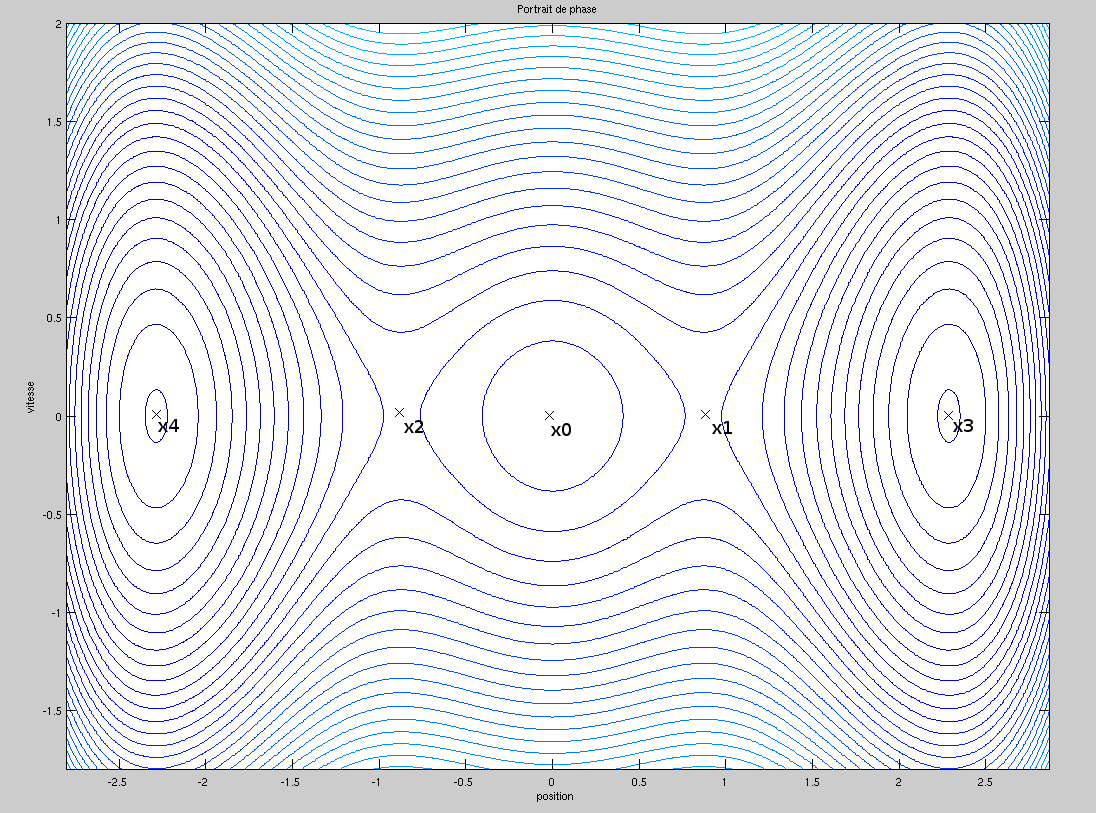
\includegraphics[scale=0.5]{PortraitDePhasePointsVisibles.png}
	\caption{Portrait de phase. $a=\sqrt{15}$}
\end{figure} 

\subsection{Que peut-on en déduire sur le mouvement.}
On remarque trois points centres en (0,0), (2.288,0) et (-2.288,0). En ces points le système est stable. Contrairement à une spirale attractive, le mouvement du pendule ne va pas ralentir mais il ne va pas non plus s'accélérer.  On remarque aussi deux points selles en (-0.874,0) et (0.874,0). En ces points le système est instable et le mouvement tend à s'accélérer en s'éloignant de cette position.%Il faudra pe modifier mon analyse.

\section{On suppose maintenant que $a=\sqrt{3}$ et $x(0)=x_0>0$ et $\dot{x}(0)=0$.}
\subsection{Calculer et représenter à l'aide de Matlab la période T en fonction de $x_0$ pour $0<x_0<10$.}
On peut déterminer la période T des oscillations en calculant cette intégrale:\\
$T=2\int_{t(x_{min})}^{t(x_{max})} dt $\\
\\
L'intégrale première du système peut s'écrire sous la forme: $ \frac{v^2}{2} + G(x) = 0 $ avec \fbox{$G(x)=\frac{1}{8}x^4 + \frac{x^2}{2} - a\sqrt{\frac{x^4}{4} + 1} $} \\
C correspond à la valeur initiale: $C=G(x_0)$ pour $x_0>0$\\
Puisque $ \frac{1}{2}\dot{x}^2(1 + x^2) + G(x) = G(x_0) $. On a alors $\dot{x} = \sqrt{\frac{2(G(x_0) - G(x))}{1 + x^2}}$\\
Connaissant $\frac{\delta x}{\delta t}$, on peut simplifier le calcul de l'intégrale pour la période T:\\
$T=2\int_{x_{min}}^{x_{max}} \frac{\sqrt{1 + x^2}}{\sqrt{2(G(x_0) - G(x))}} dx $\\
On intègre de 0 à $x_0$. On a alors:
\[\fbox{$ T=2\int_{0}^{x_0} \frac{\sqrt{1 + x^2}}{\sqrt{2(G(x_0) - G(x))}} dx $}\]
Matlab peut réaliser l'intégration. On lui demande d'intégrer sur plusieurs valeurs de $x_0$, afin de pouvoir tracer la courbe de la période en fonction de $x_0$.

\begin{figure}[H]
	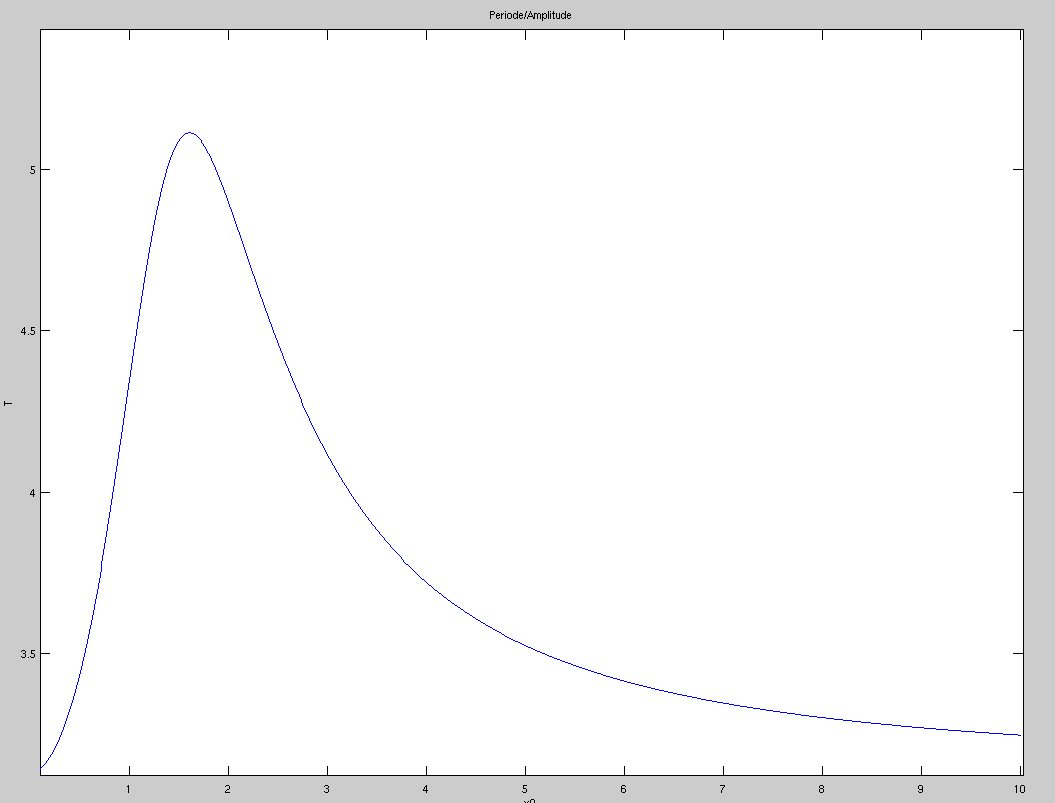
\includegraphics[scale=0.5]{PeriodePendule.png}
	\caption{Période T du système oscillatoire en fonction de $x_0$}
\end{figure} 

\section{On suppose maintenant que le système est soumis à une force de frottement $\gamma > 0$ et que l'équation devient: (E) $\ddot{x} + \gamma.\dot{x} + f(x,a) = 0$.}
\subsection{Représenter le diagramme de Matlab le diagramme de bifurcation  en $(a,\gamma)$ pour chacun des points d'équilibres.}
L'équation différentielle s'écrit désormais:\\
\[  \ddot{x} + \gamma.\dot{x} + \frac{\dot{x}^2x}{1+x^2} + \frac{1}{2}\frac{x^3}{1+x^2} + \frac{x}{1+x^2} - \frac{a.x^3}{2(1+x^2)\sqrt{x^4/4+1}}=0 \]	

Il faut calculer pour chaque points d'équilibres:\\
D= Calcul du discriminant du polynôme caractéristique\\
S= Somme des 2 valeurs propres\\
P= Produit des 2 valeurs propres \\

Pour cela, on étudie la matrice du système linéaire associée.

\[
J=
\begin{pmatrix}
\frac{\delta f_1}{\delta x_1} & \frac{\delta f_1}{\delta x_2}\\
\frac{\delta f_2}{\delta x_1} & \frac{\delta f_2}{\delta x_2} \\
\end{pmatrix}
\]

On a toujours : $\dot{x_1}=x_2=f_1(x_1*,x_2*)$\\
D'où $\frac{\delta f_1}{\delta x_1}=0$ et $\frac{\delta f_1}{\delta x_2}=1$\\
Le terme supplémentaire n'a pas une dérivée nulle par rapport à $x_2$: $\frac{\delta \gamma x_2}{\delta x_2}=\gamma$\\
Nous obtenons ainsi la nouvelle matrice Jacobienne associée au système avec forces de frottements :
\[
J=
\begin{pmatrix}
0 & 1\\
\frac{\delta f_2}{\delta x_1} & \gamma\\
\end{pmatrix}
\]
\\
$tr(J) = \gamma $\\
$det(J) = -\frac{\delta f_2}{\delta x_1} $\\
$\Delta(J) = tr^2(J)-4det(J)=\gamma^2 + 4\frac{\delta f_2}{\delta x_1}$\\ 



\subsection{On suppose que $a=\sqrt{15}$. Pour quelles valeurs (exactes) de $\gamma$ les points d'équilibres attractifs changent-ils de nature.}

Comme nous venons de le voir, en ajoutant une force de frottement, un facteur $\gamma$ est ajouté à l'équation, la trace et le discriminant sont modifiés. \\
De plus, pour les points attractifs $\frac{\delta f_2}{\delta x_1}$ < 0.\\
Nous nous intéressons donc aux trois points centres que nous avons trouvé dans les questions précédentes:\\
$x=0$\\
$x_1=\sqrt{-1+\sqrt{1+l_0^2}-\sqrt{-2-2\sqrt{1+l_0^2}+l_0^2}})$\\
$x_2=-\sqrt{-1+\sqrt{1+l_0^2}-\sqrt{-2-2\sqrt{1+l_0^2}+l_0^2}})$
\\
On étudie les signes de la trace et de Delta.\\
On détermine les racines de delta.\\
On pose:\\
$0 = \gamma^2 + 4\frac{\delta f_2}{\delta x_1}$ 
\\
$\Delta=-16.\frac{\delta f_2}{\delta x_1}$ 
\\
Les racines sont donc: $ ^+_-0.5\sqrt{\frac{-16\delta f_2}{\delta x_1}} $   Soient: $ ^+_-2\sqrt{\frac{-\delta f_2}{\delta x_1}} $  \\
On a alors le tableau de variation suivant:\\
\begin{figure}[H]
	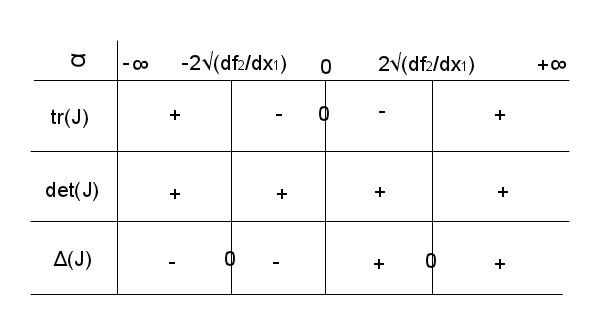
\includegraphics[scale=0.5]{tab_var_gamma.jpg}
\end{figure} 
Lorsque gamma vaut $ ^+_-2\sqrt{\frac{-\delta f_2}{\delta x_1}} $, le discriminant est nul. $x_0$, $x_1$ et $x_2$ (qui étaient des centres avant d’avoir ajouté les frottements) ne sont plus des points critiques. On constate également que de part et d’autre de ces valeurs, ces points changes de nature. Ils changent également de nature de part et d’autre de 0. A gauche de 0 ils sont attractifs et à droite ils sont répulsifs. Quant $\gamma$ vaut 0, ces points critiques sont des centres (il n’y a pas de frottement).
\\
Les points critiques attractifs changent de nature lorsque gamma vaut :\\
$ ^+_-2\sqrt{\frac{-\delta f_2}{\delta x_1}} $ ou 0. 


\subsection{Représenter le portrait de phase pour $\gamma=1, \gamma=2, \gamma=3.$}
%On calcul l'intégrale première du système afin de pouvoir déterminer le diagramme de phase. On a:
%\[\fbox{$ \frac{1}{2}v^2 + \gamma.v + \frac{1}{8}x^4 + \frac{x^2}{2} - a\sqrt{\frac{x^4}{4} + 1} = C  $}\]
L'intégrale première du système avec les frottements n'étant pas calculable, on est contraint d'utiliser la deuxième méthode pour déterminer le portrait de phase pour:\\
$\gamma=1$\\
$\gamma=2$\\
$\gamma=3$\\
La deuxième méthode permet de calculer le portrait de phase local construit à partir de solutions déterminés numériquement.  
\end{document}